\documentclass[12pt]{article}
\usepackage[utf8]{inputenc}
\usepackage{hyperref}
\usepackage{csquotes}
\usepackage{xparse}
\usepackage{graphicx}
\usepackage{xcolor} 
\usepackage{xspace}
\usepackage{listings}
\usepackage{hyperref}

% Required for specifying custom colours
\definecolor{grey}{rgb}{0.9,0.9,0.9} 


% deadline: 20.5.2021
\NewDocumentCommand{\codeblock}{v}{%
    \texttt{\textcolor{black}{#1}}%
}

\usepackage[backend=biber,
    style=numeric,
]
{biblatex}
\addbibresource{minireferences.bib}

\begin{document}
	\colorbox{grey}{
		\parbox[t]{0.93\textwidth}{ % Outer full width box
			\parbox[t]{0.91\textwidth}{ % Inner box for inner right text margin
				\raggedleft % Right align the text
				\fontsize{50pt}{80pt}\selectfont % Title font size, the first argument is the font size and the second is the line spacing, adjust depending on title length
				\vspace{0.7cm} % Space between the start of the title and the top of the grey box
				
			    The Early History of F\#\\
			   
				\vspace{0.7cm} % Space between the end of the title and the bottom of the grey box
			}
		}
	}
\\\\
\parbox[t]{0.93\textwidth}{
    \raggedleft
    Kenneth Fossen\\
    May 2021
}



\includegraphics[scale=0.75]{img/fsharp256.png}

\vfil


This essay presents the paper "The Early History of F\#"~\cite{syme_early_2020} by Done Syme~\cite{noauthor_don_2021} presented at the HOPL IV ~\cite{noauthor_hopl_nodate}.
The paper discusses the historical summary for how the F\# language was created, and how the early days functional programming (FP), and Don Syme's personal experience with FP influenced F\#'s design and implementation.
\\

I choose this paper, for a few reasons. I've been experiencing FP through other University in Bergen's (UiB) courses (INF122/22 ~\cite{noauthor_funksjonell_nodate}~\cite{noauthor_programmeringssprak_nodate}), and have been enjoying the new way of thinking and the Hindley-Miler type-inference magic~\cite{noauthor_hindleymilner_2021}.
I've also been curious to transfer this knowledge from my courses where I've been using FP, into my part-time job , where we mainly work in the imperative language C\# and .NET environment. And this paper would give me a good introduction to the language, learn it by using it, and get to understand how FP and imperative programming can inter operate in the same code base in the .NET SDK.~\cite{dykstra_net_nodate}
If I was to get to use FP in my current workplace that does .NET, this interop between C\#, F\# and .NET seems like the likely way of letting this happen, and hopefully we could harvest the best of both worlds in the software development team.
 
\newpage

\section{Brief Overview of the HOPL Paper}

The HOPL paper "The early history of F\#"~\cite{syme_early_2020} is journey of strongly typed functional programming languages in the early 80's to the creation of F\# in late 2001 and inclusion of .NET Generics in 2005. 

In this period, it covers briefly, what the basis of functional programming is, and how this inspired the paper "Why no one uses functional programming" by Philip Wadler~\cite{wadler_why_1998}. \textit{This paper was central to my understanding of the programming language landscape}\parencite[p 9]{syme_early_2020} for Don when he entered Microsoft Research in 1998. The rise of object-oriented programming (OO) that lead to Wadler and Odersky with a mission to \textit{integrate specific technical features associated with strongly typed functional languages into "mainstream" OO languages.}\parencite[p9]{syme_early_2020} that then formed the creation of Pizza programming language. This later led to Generics being incorporated in Java, and later influenced Dons work on .NET Generics~\cite{syme_ilx_2001}. This was an important inclusion in .NET as it shaped parts of F\#. 

In 2003, 0.5 version of F\# was released, but it didn't get much attention before it's F\# 1.0 in 2005. From 2001 to 1.0 the was added a many features and the language matured.
Many of the early inclusions in F\# 1.0 is today the most beloved features of the language. The Pipeline operator is one of the popular features that was added early in the language. Later Units-of-measure was added and Type Providers to mention some.

In the period 2005 $\rightarrow$ 2020, 
the paper covers the evolution of F\#, and how the industry changed and how Microsoft had to adapt to this. F\# got a new dawn with becoming open source, and cloud computing was on the rise where it played a central part.

Don also takes us through some language mistakes~\cite[p 51]{syme_early_2020} that in retrospective should not have been added to the language. Here he mentions the e.g the Back piping operator and he discusses his early F\# decision about not including, a oft-requested feature in F\# at present time, type classes that originates from Haskell.

\newpage

\section{Brief Overview of F\#}

F\# is a strongly typed functional programming language that has been heavily inspired by OCaml~\cite{noauthor_ocaml_nodate}. It started out as a project getting OCaml to run on .NET, but there was resistance in the Microsoft Research community. \textit{So, why do we really need a .NET port of OCaml? OCaml is working fine on Windows, and on many
other OS..}~\parencite[p 16]{syme_early_2020}.


But the author decided to write F\# from scratch and port the core of OCaml to target .NET.

It is strongly typed through their own implementation of Hindley Miler that works together with .NET Generics. It comes as a part of .NET SDK since 2010, and has a rich REPL through \codeblock{dotnet fsi} that supports F\# Scripting. Other tools are mentioned in section \textit{Tool Support for F\#}

Popular features of F\# is Units-of-Measure~\cite{carter_units_nodate}, Active Patterns~\cite{carter_active_nodate}, Type Providers and Quotations~\cite{carter_code_nodate}.

Units-of-Measure is type-safety for metrics. If two measures are incompatible, you e.g. can't sum them.
Also is removes any doubt about what metric this number is representing in your code. Popular example for this is NASA's Mars Climate Orbiter that failed due to a confusion between newtons and pound force.~\cite{noauthor_mars_2021}

Active Patterns allows for partial, complete and multi-case patterns.
Makes it easy to create new patterns and use them. Don's example is parsing Int and Bool in his paper. \codeblock{ let (|Int|_) str = ...}~\cite[p 29]{syme_early_2020}.

Quotation is used for Meta-programming~\cite{noauthor_metaprogramming_2021} in F\# with Abstract-Syntax Tree's (AST)~\cite{noauthor_abstract_2021} and can be used to generate code or work with language creation in F\#.

Type providers is a feature that gives strongly typed data sources.
E.g working with JSON or Databases.

NuGet~\cite{douglas_what_nodate} is the packet manager for .NET projects for C\# and F\#, and 
Since F\# is delivered through .NET SDK, you can add any new NuGet packet and start using these libraries in your code. Doesn't matter if it is written in C\# or F\#. This goes also the other way.

\newpage

\section{Pipe operator: An Overview}

It became a favorite instantly as I made me able to chain together several commands, letting it pass on the parameters from one to the next, and at the same time increased the readability. 
The operator is is just a triangle symbol \codeblock{|>}, that has the definition, where \textbf{f} is a function and \textbf{x} is a parameter.

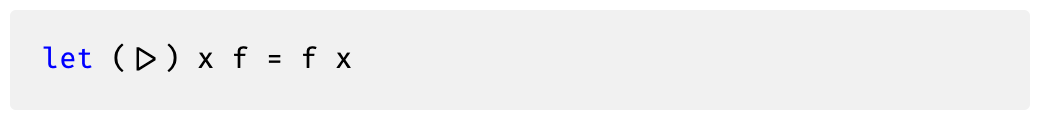
\includegraphics[scale=0.6]{img/pipeline_def.png}

From my experience with Haskell, I've come accustomed to reading from right to left in these cases, but this swap, made it intuitive and easy to read from left to right and following the logic. It's also extendable to \codeblock{||>} (two) and \codeblock{|||>} (tree parameters) to pass on to the next.
Her is a an example from the paper comparing F\# style chaining with \codeblock{|>} with Haskell style using F\#.

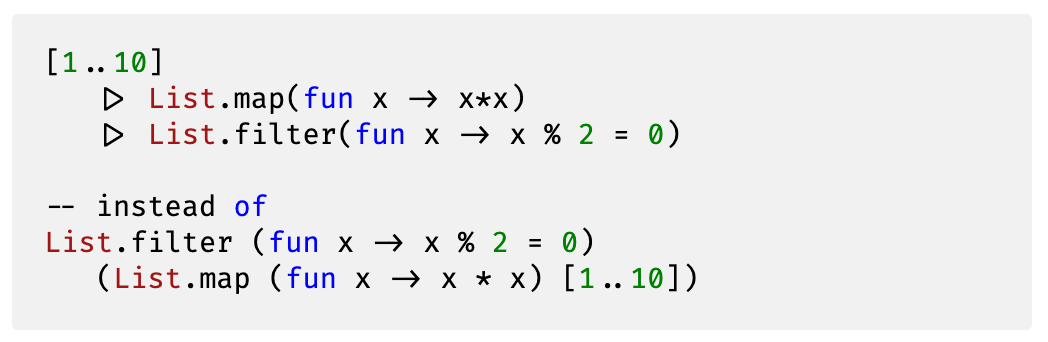
\includegraphics[scale=0.55]{img/pipeline_example.png}

The pipe operator also comes with a backward pipe operators, \codeblock{<|, <|| and <|||}.
The backward operator is not recommended to use, since it doesn't add readability for the user. This example we use the backward pipe operator. In this case we cannot chain more backward operators, due to the nature of left-to-right associating for the operator that is inherited from OCaml.

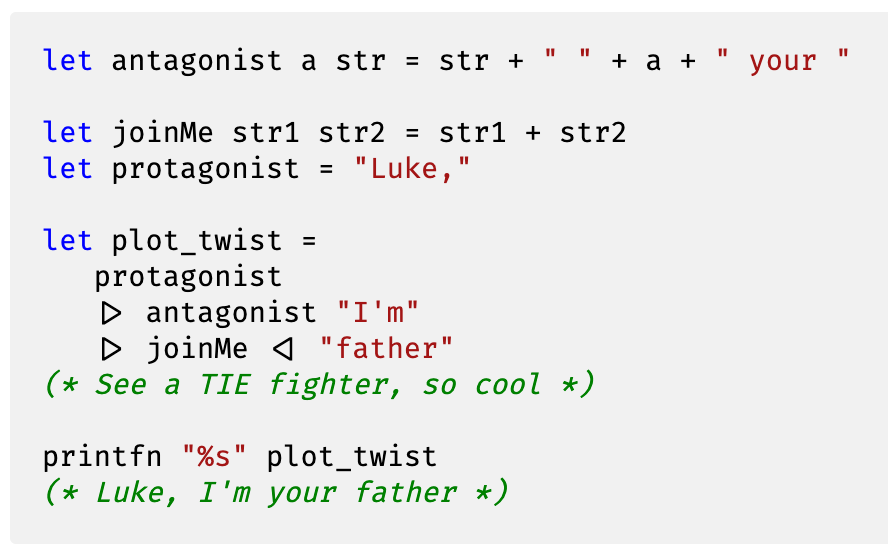
\includegraphics[scale=0.6]{img/episode5.png}

\newpage

\section{Related Work on F\#}

From the first HOPL in 1978, to the HOPL IV 2020, there has been a few contributions that link to this paper.
At HOPL I, the \textit{History of LISP}~\cite{mccarthy_history_1978} is of interest as F\# builds in these ideas that was incorporate into LISP. At the HOPL II, there was also a new contribution with regards to LISP, called \textit{The evolution of LISP}~\cite{steele_evolution_1993}. After this we can mention \textit{A history of Haskell: being lazy with class}~\cite{hudak_history_2007} that has influenced F\# design choices and is a very popular functional programming language in academia. HOPL IV, we can mention \textit{The History of Standard ML}~\cite{macqueen_history_2020} that was a direct competitor to F\# running on .NET with SML.NET port but never became anything of, and lastly \textit{A History of Clojure}~\cite{hickey_history_2020} that is a functional dialect of LISP interacting with Java that is sharing some of the same ideas of F\#.\\

Related work that paved the road for F\# to integrate with .NET is the authors work on .NET Generics.~\cite{syme_ilx_2001}. Besides this, \href{https://fsharp.org}{fsharp.org} is a good starting place for more information about the language itself, community and many other resources. One part of this website is 
\href{https://fsharp.org/teaching/research.html}{Academic Papers} page that contains a list of academic publications that could be of interest for the reader to study up on.
Furthermore you can follow their work on their GitHub account \href{https://github.com/fsharp}{github.com/fsharp}. \\

\section{Tool Support for F\#}
The great thing about F\# is that is runs everywhere the .NET SDK~\cite{dykstra_net_nodate} is installed.
This means you can use \codeblock{dotnet} too that comes with the .NET SDK to create projects.
But this is not the only way to use F\#. It is easy to follow F\# guides on Microsoft's web pages~\cite{carter_get_nodate} with F\# Scripting (\textit{.fsx}) and use either VSCode~\cite{microsoft_visual_nodate} or your favorite editor.
VSCode supports the community created Ionide extention~\cite{noauthor_ionide_nodate} that gives good language support for F\#. The REPL that follows .NET SDK, I found not useful and I would stay away from it, due to its cumbersome addition of double \codeblock{;;} for commands and other quirks from the OCaml notation.
I mainly used VSCode with Ionide, but I will also highly recommend JetBrains Rider~\cite{jetbrains_rider_nodate} with .NET development.


\section{Personal Experience}

In the paper, I really enjoyed how Don Syme took us through the history from the early 70's of FP to the inspiration for how and why F\# was created. It was exciting to see what inspired and what other languages influenced Don before he created this language. My limited use of the language has shown me a positive side of the F\# language, though I struggle some with things, when moving from Haskell world. I look forward to try to incorporate this language into my work, and here I believe Units-of-Measure is a big thing we could benefit from.


One of the things I struggle with in F\# was getting going, F\# Scripting is one thing, modules and projects are another. Why can't we just use them straight up as we can in Haskell? 
Since C\# put a lot of restrictions on how they did things in F\#, I'm curious to ask, how the author would have seen F\#'s if it wasn't so tied to C\# and their development? Also the author mentions that \codeblock{Span} helped iron out some minor problems since F\# 2.0. Are there other aspects of C\# and/or .NET that is hindering F\# move in the direction that would make F\# more adaptable and usable? 

\newpage
\printbibliography
\end{document}